\documentclass[12pt]{article}

% House style preamble
\input{.house-style/preamble.tex}

% TikZ for the threat-structure DAG (Section 5)
\usepackage{tikz}
\usetikzlibrary{arrows.meta, shapes.geometric}
\usepackage{placeins}
\usepackage{amsmath}

% --- Anonymization toggle for double-blind review ---
% Default build (make / make quick): full manuscript with the author block.
% Blinded build (make blind): author name, ORCID, affiliation, and contact
% removed. Triggered by \blindbuild, passed on the command line by the Makefile.
\newif\ifblind
\ifdefined\blindbuild \blindtrue \else \blindfalse \fi

\hypersetup{
  pdftitle={Did the intervention change usage? Validity threats and difference-in-differences in before-and-after corpus designs},
  pdfkeywords={construct validity, difference-in-differences, causal inference, corpus composition, research methods, language policy evaluation}
}
% In blind mode, strip the author from the PDF metadata too: the house-style
% preamble hardcodes pdfauthor={Brett Reynolds}, so this override must follow it.
\ifblind\hypersetup{pdfauthor={}}\fi

\title{Did the intervention change usage?\\
{\large Validity threats and difference-in-differences in before-and-after corpus designs}}
\ifblind
  \author{[\textit{Author name, ORCID, and affiliation removed for double-blind review}]}
\else
  \author{Brett Reynolds \orcidlink{0000-0003-0073-7195}%
  \thanks{Contact: \href{mailto:brett.reynolds@humber.ca}{brett.reynolds@humber.ca}}\\
  Humber Polytechnic \& University of Toronto}
\fi
% Set to the submission month. Frozen rather than \today so the date doesn't float per build.
\date{July 2026}

\begin{document}
\maketitle

\begin{abstract}
Researchers routinely claim that a policy, reform, or campaign changed language use, comparing corpus frequencies before and after. A corpus frequency is a score, not the construct it stands for: it carries the population rate plus whatever the corpus's composition and coding contributed. That contribution shifts across periods for reasons unrelated to anyone's usage, and a two-point comparison can't separate it from an effect. Difference-in-differences is the standard repair, and this paper translates its assumptions into corpus terms. Parallel trends then have to hold twice, in the underlying rate and in the corpus itself. A worked case shows the first holding exactly while the second fails, producing a four-point effect where the true effect is zero. Diagnostics can disqualify or bound a causal reading, never confirm it. The paper supplies a reporting standard and a pre-specified decision procedure ending in one of four verdicts, one of which is that the effect isn't identified, with simulations mapping where the procedure works. Feminization of profession nouns under francophone language policy is a stress test, not a finding.
\end{abstract}

\noindent\textbf{Keywords:} construct validity; difference-in-differences; causal inference; corpus composition; research methods; language policy evaluation

\section{The problem}
\label{sec:problem}

A researcher wants to know whether something worked. A language policy, a curriculum reform, a public campaign, an editorial standard. The intervention has a date, usage before and after it can be counted in a corpus, and the counts have moved. The difference looks like the effect.

It rarely is, and the reason is a measurement problem before it's an estimation problem. A corpus frequency is a score, and like any score it stands in for a construct it doesn't equal. Validity theory names two ways a score can fail the construct it's meant to represent: \term{construct underrepresentation}, where the measure captures less than was intended, and \term{construct-irrelevant variance}, where the measure moves for reasons that have nothing to do with the construct \citep{messick_1989_validity,messick1995Validity}. A corpus frequency carries both. The second is what breaks before-and-after designs. The sources a corpus draws on shift over time, so the construct-irrelevant part of the score doesn't sit still: it moves systematically from one period to the next, in the same direction, and for reasons no reader of the counts can see. A two-point comparison can't separate that movement from the effect the researcher is after.

Corpora are built in a way that guarantees the movement. A corpus isn't a sample of a population's usage; it's a sample of texts, gathered by editors and archivists whose priorities shift \citep{biber1993}, so balance and representativeness are approximations rather than guarantees \citep{McEneryHardie2012}. Diachronic work compounds it, because a matched corpus has to hold its sampling frame steady while the genres inside it drift \citep{LeechHundtMairSmith2009}. So a corpus frequency carries two things at once, what the target population did and what the corpus contributed, and the DiD machinery has to be told which of them it's being asked to identify.

The causal reading enters easily all the same, often through a verb, usage that \mention{responds to} a reform rather than an argued claim. Researchers working on prescription have long felt this pull: confronting normative dictates with usage, it tends to find the causal link assumed rather than demonstrated, from relativizer choice in edited English prose \citep{HinrichsSzmrecsanyiBohmann2015} to five centuries of French injunction set against the record of speech \citep{PoplackDion2009}. One robustness check is grammatical. Delete the causal verb and see what claim is left.

A rise after an intervention is a correlation in time. What licenses a causal reading is a design, and the standard design for this situation is difference-in-differences (DiD): set the treated series against a comparison series the intervention left untouched, and read the effect off the change in their gap. That reading rests on one assumption, called \term{parallel trends}: absent the intervention, the two series would have moved together, so the comparison series stands in for what the treated series would have done.

Because the outcome is a score rather than the construct, the assumption has to hold twice. The rate at which people use the form has to move in parallel across the two series, and so does whatever the corpus itself contributes to the score. Section~\ref{sec:estimand} works this through in numbers: the first can hold exactly while the second fails, and the failure alone produces a four-point effect where the true effect is zero. Causal inference from text is an active field \citep{keith2020text,grimmer2022text,egami2022texts}, but it has mostly handled text as a treatment, outcome, or confounder in a cross-section. Less settled is what DiD's assumptions become when the outcome is a corpus frequency measured across time.

The contribution is a discipline for claiming with DiD, not a tutorial on running it; the econometric side already has a current practitioner's guide of its own \citep{BakerEtAl2026}. A before-and-after corpus contrast supports a causal reading only after three things have been pulled apart: what population the claim is about, what the corpus's composition contributed, and what the measurement procedure contributed. A second separation, among the units at which language varies, at which treatment varies, and at which observations stop being independent, is set out in Section~\ref{sec:estimand}. Conflate any two and the apparent effect can be an artifact of the corpus, not a fact about the language.

Language research has spent a decade on reproducibility, replicability, and robustness, corpus work included \citep{SchweinbergerHaugh2025,Flanagan2025}. That programme asks whether a descriptive estimate survives reanalysis, resampling, and analytic choice \citep{EgbertBiberGrayLarsson2025,Sonning2024}. The question here sits in front of it: whether a before-and-after contrast licenses a causal reading at all. A result can be perfectly reproducible and still identify nothing.

Seven questions drive the paper, and the sections take them in turn. What's the shock, and at what unit does treatment vary (Sections~\ref{sec:estimand} and~\ref{sec:treatments})? Which population rate is the target, and what outcome measures it (Sections~\ref{sec:estimand} and~\ref{sec:outcomes})? What comparison makes the counterfactual plausible, what corpus-specific threat could counterfeit the effect, and what diagnostic would expose it (Sections~\ref{sec:threats} and~\ref{sec:diagnostics})?

The running case is the feminization of profession nouns under francophone language policy \citep{Fujimura2005,BurnettBonami2019}. It's a teaching vehicle, not a finding: the aim is the method, and the case is built so that its verdict is sometimes that the effect can't be identified. A corpus DiD is worth most when it disciplines a causal claim downward, and that's the argument the rest of the paper makes.

\section{The DiD estimand in corpus terms}
\label{sec:estimand}

DiD asks one question: across a shock, did the treated series and a comparison series no shock touched change differently? Take the treated variety's before-to-after change in the outcome, subtract the control's, and under a single assumption (that absent the shock the two would have moved in parallel) the remainder estimates the average treatment effect on the treated (ATT) \citep{RothSantAnnaBilinskiPoe2023}.

Say feminine marking rose twelve points in the treated variety across the window and five in the comparison: DiD reads the policy effect as the seven-point excess, on the assumption that without the policy the treated variety would have risen by the same five. Everything corpus-specific lives in what fills \enquote{outcome} and \enquote{series}.

That last clause is where the canonical panel idealization, the clean grid of the same units measured period after period, breaks down for a corpus as for any constructed aggregate. What a finite corpus yields is a realized sample proportion $\hat f$; the quantity of interest, the estimand, is the latent rate $\pi$ at which a specified population uses the form in a specified context, for the running case the share of profession- and title-noun tokens with a female referent that take feminine marking, in a named text population.

Let $f$ be the expected corpus frequency: the proportion induced by the corpus and coding process before sampling noise. Then $\hat f = f + \epsilon$ and $f = \pi + b$, with $b$ collecting composition (whose texts, which genres, what topics) and measurement (how the form was coded or transcribed). $b$ is the construct-irrelevant part of Section~\ref{sec:problem}, written as a quantity: the amount by which the corpus's own construction moves the score away from the rate the claim is about.

Feminine marking can climb in the corpus series with no change in anyone's usage at all: a paper that runs more profiles of women in the professions, or a transcription service that starts spelling out feminine titles it used to abbreviate, moves $f$ while $\pi$ holds still. Read $b$ as the gap itself, $b = f - \pi$: not a random error that more data averages away, but whatever composition and measurement added, fixed once the texts and the coding are.

Collecting more tokens shrinks $\epsilon$ around $f$ without touching $b$; the cell-level uncertainty of Section~\ref{sec:modern} stays separate from $b$, the corpus filter: the standing contribution the corpus's own construction makes to the score. The outcome estimated from the page isn't the quantity the claim is about.

Differencing doesn't remove $b$ either. The mechanism is easiest to see away from the running case, where the numbers can be chosen rather than estimated, so take a curriculum reform in one region's schools, textbook corpora sampled before and after, and a second region with no reform as the comparison. Suppose the feature of interest runs at 10\% in science textbooks and 30\% in language-arts textbooks before the reform, and that it rises by two points in both subjects, in both regions, across the window. Usage is genuinely changing, and changing identically on the two sides, so the reform's true effect is zero. Suppose too that publishers in both regions were moving their lists toward language arts over these years, and that the treated region's collection followed further than the comparison region's: science falls from half the corpus to a fifth there, and from a half to two fifths in the comparison (Table~\ref{tab:composition-artifact}).

\begin{table}[!ht]
\centering
\footnotesize
\caption{Composition drift manufacturing a difference-in-differences effect. The feature runs at 10\% in science and 30\% in language arts before the reform and rises two points in both subjects, in both regions, so the reform's true effect is zero and the true rate rises in parallel on the two sides.}
\label{tab:composition-artifact}
\begin{tabular}{@{}l c c c@{}}
\toprule
 & Science share of corpus & True rate & Observed rate \\
\midrule
Treated, before    & 0.50 & 0.200 & 0.200 \\
Treated, after     & 0.20 & 0.220 & 0.280 \\
Comparison, before & 0.50 & 0.200 & 0.200 \\
Comparison, after  & 0.40 & 0.220 & 0.240 \\
\bottomrule
\end{tabular}
\end{table}

The true rate rises two points on both sides, so parallel trends holds in the quantity the claim is about, and holds substantively rather than by both series standing still. The observed treated series nonetheless rises eight points against the comparison's four, and DiD reports the four-point excess as the reform's effect. There was no effect; every point of it is $b$.

This is aggregation bias with a time dimension, Simpson's paradox in a panel, and it's worth naming as such rather than presenting the mechanism as new. What makes it a corpus problem is who sets the weights. The researcher doesn't choose the mix: archivists, publishers, and digitization projects do, across decades, for reasons that have nothing to do with any study.

Two separate things follow, and they're easy to run together. The \emph{diagnostic} is to compare the composition margins across the series: a science share that moved thirty points on one side and ten on the other already puts parallel trends in $b$ in doubt, and that comparison needs no knowledge of the true effect. The \emph{repair} is to standardize both series to a common composition before differencing, which here returns exactly zero, and returns zero for any reference mix.

The example is deliberately the easy case, because subject area is recorded and can be reweighted. Where composition moves on a margin the metadata doesn't carry, the same arithmetic runs and neither the diagnostic nor the repair is available. Differencing removes whatever the two series share, so it removes the level of $b$ and any drift common to both; what it can't remove is a \emph{differential} drift, which is set by the archives rather than by the language.

The residual isn't empty. Stratify the texts by the margins composition moves on (outlet, profession, topic). Within each stratum $s$, let $\pi_s$ be the true rate, $r_s$ the rate the corpus records, $q_s$ the corpus's share of $s$, and $p_s$ the target population's. Then $f = \sum_s q_s r_s$ and $\pi = \sum_s p_s \pi_s$, so

\[
b = \underbrace{\sum_s (q_s - p_s)\,\pi_s}_{\text{composition}} + \underbrace{\sum_s q_s\,(r_s - \pi_s)}_{\text{measurement}}.
\]

Reweighting sets $q_s$ to $p_s$ on the strata it can see, zeroing the first term; the second survives. The part of it the strata are too coarse to resolve is the hidden drift of Section~\ref{sec:worked}, and the simulations are built on this split.

Differencing is linear, so the DiD of the expected corpus frequency separates into the DiD of $\pi$ and that of $b$, $\mathrm{DiD}(f) = \mathrm{DiD}(\pi) + \mathrm{DiD}(b)$. The first term, under parallel trends in the rate, is the target effect. For a usage-rate estimand, the second is contamination, and it vanishes only under a second parallel-trends assumption, $\mathrm{DiD}(b) = 0$: that composition and measurement would have drifted alike in both series.

A corpus design needs parallel trends twice over, in $\pi$ and in $b$, where the canonical panel setting quietly assumes the second away.

Readers who work with tests and scales have met this requirement before, under another name. Comparing group means on an instrument presupposes \term{measurement invariance}: that the instrument relates to the construct the same way in each group, so a difference in scores is a difference in the thing measured and not in how it was measured \citep{meredith1993measurementInvariance,millsap2011measurementInvariance}. Without invariance the comparison isn't interpretable, however large the samples. Parallel trends in $b$ is that requirement moved from groups to periods and from levels to changes: the corpus has to relate to usage the same way on both sides of the contrast, or at least depart from it in the same direction and degree. A corpus assembled differently before and after the shock is a scale rescored between administrations. Picture one variety's archive getting re-digitized and re-tagged halfway through the window while the other's is left alone: the two corpora's coding has now drifted apart even if actual usage tracked perfectly, and that drift would enter the estimate as if it were the policy's effect.

Both are claims about an unobserved counterfactual: pre-treatment comparisons can discredit them but can't verify them. And since only $\hat f$, an estimate of $f$, is observed, a flat pre-period in the observed series is consistent with non-parallel trends in $\pi$ and in $b$ that cancel, so the pre-period tests the two assumptions jointly, never apart.

Neither half is optional, and the temptations run both ways. Once the composition term is on the table it's easy to treat it as the whole problem and forget the ordinary assumption about the rate; it's equally easy to wave at adjusting for composition and assume the rate takes care of itself. Both shortcuts fail. The observed contrast recovers the effect on $\pi$ only when the rate would have moved in parallel \emph{and} the bias would have moved in parallel.

One refinement decides how the corpus-filter term is handled, turning on which effect is wanted. The filter reaches the observed contrast two ways: a non-policy drift, which the second assumption requires to be parallel, and a policy-induced shift, the policy changing what gets written rather than how a given referent is marked.

For an effect on the usage rate $\pi$, that second shift is nuisance as well, even though the policy caused it: a topic or profession mix that moved gets reweighted to a fixed mix, isolating the marking rate. The other estimand, sometimes the one actually wanted, is the policy's total effect on the observed output. It keeps the writing that the policy moved, so that same shift is part of the answer, and reweighting it away would subtract a piece.

The two estimands differ exactly by the policy-to-composition path, and a design that doesn't say which it means can defend neither. The one margin neither estimand touches is the outcome margin itself: the realization strategy of Section~\ref{sec:outcomes}. Condition there and the effect itself is removed.

Naming the estimand forces apart five units a corpus invites running together. The \term{linguistic unit} is the variable whose rate is at issue (feminine marking of a profession noun for a female referent). The \term{measurement unit} is what gets counted to estimate that rate (eligible tokens, or documents). The \term{aggregation unit} is the cell those counts are summed into before estimation (an outlet-month, a title-variety-year), which sets the weights and denominators and can quietly change the estimand.

The \term{identifying unit} is where the treatment varies (the variety or polity). The \term{dependence unit} is the level at which residuals correlate and inference is clustered, here the variety again; with only a few varieties the usual large-sample standard errors don't hold, which is the inference problem Section~\ref{sec:modern} takes up.

Merging them is dangerous because the five sit at wildly different scales. A corpus offers millions of measurement units and, often, two or three identifying units; the latter govern how much can be concluded. Counting tokens as though they were the sample size manufactures a precision the design doesn't have \citep{BertrandDufloMullainathan2004}: it's like claiming a hairline margin of error on a two-person poll because each person answered a thousand questions.

Here, the target is the effect on $\pi$; the price is parallel trends in both $\pi$ and $b$. The diagnostics of Section~\ref{sec:diagnostics} can falsify that assumption or bound how far it may fail, never confirm it, and Section~\ref{sec:worked} puts the discipline to work, each design declaring its estimand in a ledger (Table~\ref{tab:ledger}) before anything is estimated.

\section{What counts as treatment in language data}
\label{sec:treatments}

In a policy evaluation the treatment is usually a known act on a known date: a law takes effect, a price changes, a program opens. Language data rarely offers that. A change in usage may be pushed by a circular, a dictionary, an administrative endorsement, a first enforcement, a media house revising its style sheet, or a social movement that made all of these possible. Which act counts as the treatment isn't given by the corpus; it fixes the estimand.

The shock need not be a policy. It can be a new medium with constraints of its own, a contact or demographic event, a censorship regime imposed or lifted, or a non-linguistic event that drags vocabulary behind it. These can be cleaner than decrees because their timing is less likely to be chosen by the speech community. The policy case this paper uses is the demanding one: a decree's timing may be bound up with the trend it's meant to explain.

The feminization case shows the ambiguity. Candidate treatments include an endorsement, a feminized-titles dictionary \citep{Moreau1991}, a circular, and the date editors actually began applying the forms. France's 1986 circular \citep{france1986circ} urged feminine titles and went largely unenforced, by the government's own later admission, until a second circular in 1998 \citep{france1998circ,BurnettBonami2019}. Those two acts share their text and differ in force, which makes 1986 useful as a near-null policy: a case that should show little or nothing, not a failed treatment.

Official dates can also lag the changes they name. An endorsement often ratifies a shift already under way rather than starting it, a question of actuation \citep{BurnettBonami2019}. Feminization is a socially structured diffusion, an S-curve spreading token by token and register by register \citep{weinreich1968,tagliamontedarcy2007}.

Two varieties can both be rising and still violate parallel trends if one is in the steep middle of its curve and the other is leveling off. A shock identifies an effect only when it appears as a level shift or acceleration on top of comparable untreated trajectories; otherwise \enquote{not identified} is a property of the design, not a disappointment after estimation.

Treatments in this domain are rarely binary either. Endorsements vary in scope and force, so two polities labelled treated may have received different doses. Where dose is measurable, intensity is more honest than an on-off indicator; where it isn't, the binary coding is an assumption to report.

The boundary also leaks: a policy in one polity reaches readers in another through shared media and the channels opened by a common language. The first question of a corpus DiD is this: which act, at which date, with what force and reach, is being called the cause. The estimand, comparison, and diagnostics inherit that choice.

\section{Outcome construction}
\label{sec:outcomes}

A corpus outcome is transparent when anyone could reproduce it from the same texts by a stated rule: a count over forms, a closed-set alternation, a tagged feature. It's model-dependent when a classifier, parser, or embedding stands between the text and the number. Both are usable, but they fail differently.

A transparent count errs in what its rule misses; a model-dependent measurement adds the model's own drift, which can move with the period or variety under study and so mimic the effect. The check is differential: a classifier or parser has to be evaluated by period and by variety, since an error rate that holds on average but shifts across the window is the measurement twin of a non-parallel trend.

Because the outcome is a proportion, measurement bias is level-dependent even at fixed error rates. It tracks $\pi$ itself, so a moving rate drags the filter through the measurement model. A classifier that mislabels one token in twenty both ways doesn't add a flat five-point bias: a true rate of ten percent reads as fourteen, a true ninety as eighty-six, and a true fifty as fifty. The two parallel-trends assumptions are coupled in mechanism, not only in the data.

A second choice hides inside the first. Most variables of interest are realized in more than one way, and a single count silently treats those ways as exchangeable signs of one change. Feminine marking for a woman can surface as a distinct noun form (\mention{autrice}), as feminine article or agreement on an otherwise invariant noun (\mention{la ministre}), or as both. Pooling them assumes the realizations rise together; breaking the outcome out by strategy tests that assumption, especially because varieties favour different strategies \citep{Dawes2003}.

The marker also needs its conditioning fixed. A feminine article counts as feminization only when the referent is independently known to be a woman, so the outcome definition carries that conditioning rather than assuming it. Agreement already at ceiling is noise, not outcome; the informative cases are the contested ones, such as feminine marking on default-masculine or epicene titles.

Breaking the outcome out by strategy diagnoses the pooling assumption without fully replacing it. Separate strategy-specific analyses show which realization moved, but they treat mutually exclusive choices as independent outcomes and discard substitution among them. The fuller treatment models realization as one categorical outcome, letting the strategies compete within one estimator, as \textcite{Xu2017} develops for categorical outcomes in regression discontinuity. This paper stops at decomposition: a joint categorical DiD is a natural next step, not a claim made here.

Finally, a proportion needs a denominator named as carefully as the numerator. Feminine-marked tokens can be counted against every profession noun, only female-referent tokens, or only title-address contexts. Weights can attach to tokens, documents, or title-variety cells, and the referent distribution may itself be moving. The numerator is visible. The denominator is where composition re-enters.

\section{Identification threats specific to corpora}
\label{sec:threats}

The threats a corpus DiD faces are easiest to read off a small set of causal paths (Figure~\ref{fig:threat-dag}; read each arrow as \enquote{this directly affects that}). They fall into five families: composition, measurement, interference, aggregation, and selection into treatment timing. The first four are inflected, or created, by the corpus; the fifth is the ordinary confounding worry any DiD faces. Each is a way the observed contrast can be mistaken for the policy's effect on the population rate.

\begin{figure}[t]
\centering
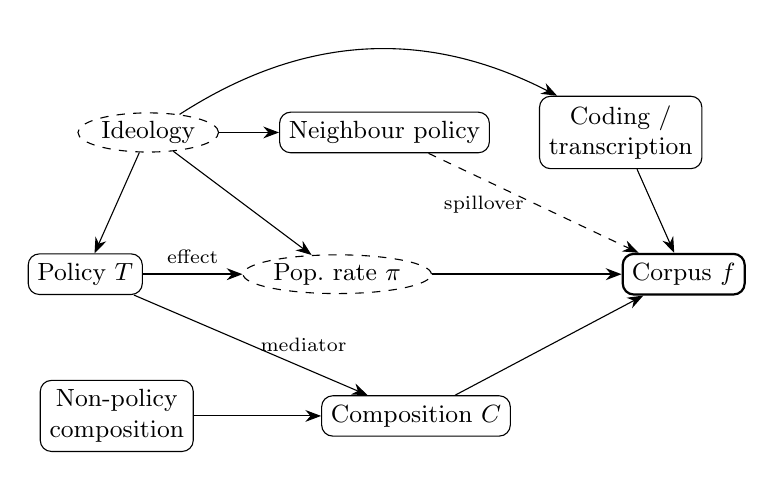
\begin{tikzpicture}[>={Stealth[length=2mm]}, every node/.style={font=\small, align=center}]
  % top row: ideology and the children that reach f without passing through pi
  \node[draw, dashed, ellipse, inner sep=1pt] (I)  at (1.6,1.8)   {Ideology};
  \node[draw, rounded corners]                (Tn) at (4.6,1.8)   {Neighbour policy};
  \node[draw, rounded corners]                (M)  at (7.6,1.8)   {Coding /\\transcription};
  % middle row: the causal spine
  \node[draw, rounded corners]                (T)  at (0.8,0)     {Policy $T$};
  \node[draw, dashed, ellipse, inner sep=1pt] (pi) at (4.0,0)     {Pop.\ rate $\pi$};
  \node[draw, thick, rounded corners]         (f)  at (8.4,0)     {Corpus $f$};
  % bottom row: the composition layer
  \node[draw, rounded corners]                (Sc) at (1.2,-1.8)  {Non-policy\\composition};
  \node[draw, rounded corners]                (C)  at (5.0,-1.8)  {Composition $C$};
  \draw[->] (I) -- (T);
  \draw[->] (I) -- (pi);
  \draw[->] (I) -- (Tn);
  \draw[->] (I) to[bend left=30] (M);
  \draw[->, thick] (T) -- node[above, font=\scriptsize] {effect} (pi);
  \draw[->] (T) -- node[midway, right, font=\scriptsize] {mediator} (C);
  \draw[->] (Sc) -- (C);
  \draw[->, thick] (pi) -- (f);
  \draw[->] (C) -- (f);
  \draw[->] (M) -- (f);
  \draw[->, dashed] (Tn) -- node[below left, font=\scriptsize, pos=0.5, yshift=6pt] {spillover} (f);
\end{tikzpicture}
\caption{The causal paths a corpus DiD contends with: a threat map, not a graph that identifies the effect. Dashed nodes are unobserved. The heavier spine marks the target route from policy to population rate $\pi$ to corpus frequency $f$; the other paths mark composition, measurement, interference, and ideology-driven timing threats. Parallel trends itself isn't a path in a static graph.}
\label{fig:threat-dag}
\end{figure}

Composition splits in two. A policy can move the mix it's measured against, the professions in the news or the topics in play, so part of composition lies on the path from treatment to $f$ (the edge $T \to C$). Whether to reweight it away depends on the estimand: for a usage-rate effect it counts as nuisance; for a total-output effect it belongs to the answer.

Non-policy composition drift, such as outlet entry, author turnover, or register mix, is a bias source either way. The two look alike in the data, so the margins to reweight have to be named before the estimate is seen.

Measurement is the second. What the corpus records isn't the latent rate but a coding of it, and the coding can drift: a classifier whose error rate moves with the period, a transcription house style that adopts new forms on a date of its own. When it does, $f$ jumps while $\pi$ holds still. The instrument measuring the outcome has become a moving part \citep{keith2020text}.

Interference breaks the assumption that one variety's treatment leaves the others untouched. Suisse romande shares wire services with France; the same dictionaries and style guides circulate across the francophonie; writers file across borders. A not-yet-treated control is then lightly dosed. Shared wire copy can be held aside and deduplicated; the other channels can't, so the estimand has to name whether it seeks the policy's direct effect net of diffusion or its total effect including it.

Aggregation is the easiest to overlook. The level at which counts are summed into observations (token, document, outlet-month, title-variety-year) fixes weights and denominators. A few prolific outlets or a burst of one topic can carry a token-level rate that a cell-level rate wouldn't. The aggregation unit is a modelling choice with identifying consequences, not bookkeeping.

Selection into treatment timing is the deepest threat, and it's the corpus form of a problem that recurs wherever a comparison group has to stand in for a counterfactual rather than being assigned to it \citep{OlsonDoyleJiang2026}. A polity tends to legislate when its gender politics have already moved, and that same movement shifts usage, so adoption timing is correlated with the outcome's trajectory. No estimator removes that fork; in a two-group design it's observationally indistinguishable from a real effect.

That last threat is where the figure reaches its limit. A graph can inventory paths, but identification turns on a counterfactual trend: whether usage and the corpus filter would have moved in parallel absent the policy. The diagnostics, not the diagram, carry that weight.

\section{Diagnostics}
\label{sec:diagnostics}

A diagnostic here does two things and not a third. It can disqualify a causal reading, or bound how far the identifying assumption may bend before the result flips. It can't confirm parallel trends, since the counterfactual it concerns is never observed. Diagnostics are pre-specified tests, not a checklist run after the estimate to bless it. What has to be on the record before any of them runs is set out in Table~\ref{tab:reporting}.

The discipline starts before any test, with the roles. Each textual feature should be assigned a job: does it measure the outcome, identify the referent that conditions the outcome, index composition, or sit downstream as part of the outcome itself? No feature can hold two of these jobs at once. Conditioning on a downstream realization strategy subtracts the effect; conditioning on a drifting measurement cue imports drift; and reweighting follows from the declared estimand.

\begin{table}[t]
\centering
\footnotesize
\caption{Minimum report for a corpus DiD. The point is to make the identifying claim auditable before the estimate is read.}
\label{tab:reporting}
\begin{tabular}{@{}p{0.28\textwidth} p{0.64\textwidth}@{}}
\toprule
\textbf{Item} & \textbf{What to state} \\
\midrule
Estimand & population usage rate, corpus-output effect, or design contrast \\
Treatment & act, date, force, timing theory, and expected sign \\
Target population & variety, register, period, conditioning context, and denominator \\
Composition margins & margins fixed, reweighted, left in the estimand, or unavailable \\
Measurement audit & coding, transcription, or classifier checks by period and series \\
Identifying unit & unit where treatment varies, such as polity, variety, outlet, or platform \\
Dependence unit & level for clustering, randomization, or uncertainty reporting \\
Interference check & shared source, wire copy, exposure, or diffusion diagnostic \\
Sensitivity benchmark & pre-specified plausible violation of parallel trends \\
Permitted verdict & \term{bounded estimate}, \term{descriptive reading}, \term{shared wave}, or \term{not identified} \\
\bottomrule
\end{tabular}
\end{table}

The first diagnostic family tests the pre-period. Event-study estimates against not-yet-treated comparisons \citep{SunAbraham2021,BorusyakJaravelSpiess2024} show whether the series moved together before the shock, but a flat pre-period only fails to discredit parallel trends \citep{RothSantAnnaBilinskiPoe2023}. The sharper question is onset versus acceleration: does the marking rate change at the treatment date, or was the divergence already under way?

That distinction is easy to nod at and hard to hold onto, so it's worth naming the two ways a clean pre-period misleads. The first is cancellation. What the pre-period exposes is $\hat f$, which carries $\pi$ and $b$ together; a usage rate drifting up in the treated series and a composition drifting down can sum to a flat line. Flatness then reports that two movements happened to offset, not that neither occurred. The second is timing. Nothing obliges a confound to announce itself early, and the ones that worry a corpus analyst rarely do: an archive re-digitized in the year of the reform, a wire service taken on at the same moment, a publisher's list that turned when the policy did. Drift that begins where the test stops looking leaves no pre-period signature at all.

So a pre-period test is a screen, not a licence, and the asymmetry should be visible in how the result is written. Failing it is close to decisive. Passing it is weak evidence, and it belongs in the report as a check that didn't fire rather than as grounds for believing the assumption holds.

The second family breaks the design on purpose. A placebo date, a near-null policy used as a negative control, or a shuffled treatment label should return nothing. With a handful of identifying units, these permutations calibrate the size of contrast the procedure can manufacture; they aren't a $p$-value from an assignment that was never random \citep{BertrandDufloMullainathan2004}.

The third family withholds parts of the corpus. Leave-one-source-out re-estimation asks whether the effect lives in the whole series or in one outlet, author, region, wire feed, or burst of reprinted copy. An estimate carried by one source is idiosyncrasy or interference, not an effect.

The fourth family probes the corpus filter. Reweighting to a fixed composition removes a measured artifact on pre-committed margins; policy-moved mix is reweighted away for a usage effect and kept for a total-output effect. Re-running the analysis strategy by strategy is the parallel outcome check: if low-cost agreement and high-cost derivation move differently, the assumption that they're exchangeable signs of one change has failed.

The last family quantifies fragility. Rather than assert parallel trends, sensitivity analysis asks how large a violation would have to be to overturn the result and compares that breakdown value to a pre-specified benchmark, such as the largest trend swing in an untreated stretch or untreated variety \citep{RambachanRoth2023}. A result that survives only a smaller violation hasn't earned its causal claim; one that survives a larger violation earns a bounded claim, reported as a sensitivity interval, not a point.

The benchmark has a blind spot: it sees only violations that leave a footprint in the windows used to build it. Drift confined to the treated post-period can clear the bar untouched, which is the failure the simulations of Section~\ref{sec:worked} quantify. The resulting claim is bounded against named and benchmarked confounds, not against every possible one.

The checks feed one rule. A date-aligned divergence that survives composition, interference, onset, and sensitivity checks licenses a \term{bounded estimate}, scoped to the register measured. A divergence leaning on an ambiguous check licenses a \term{descriptive reading}. Calendar-time co-movement with no date-aligned divergence is a \term{shared wave}. A pre-treatment divergence, an effect carried by shared-source material, unanswerable selection into timing, or a breakdown value below a plausible confound forces \term{not identified}. The ladder's point is that a downgrade is a result: a corpus DiD succeeds when it returns the right verdict, not when it returns an effect.

Stated that way the rule is a policy, not yet a procedure. What makes it operable is fixing each gate's statistic and its threshold before the data is seen. Table~\ref{tab:gates} gives the instantiation used for the worked example, the same logic all three simulation scripts apply.

\begin{table}[!ht]
\centering
\footnotesize
\caption{The automated gates, in order, as applied by all three simulation scripts. The first gate to trip decides. Thresholds were fixed against the design before any run; the placebo band is calibrated from the data rather than chosen. Gate~2 branches rather than deciding, and two of the four permitted verdicts are out of reach here.}
\label{tab:gates}
\begin{tabular}{@{}l p{0.34\textwidth} l p{0.28\textwidth}@{}}
\toprule
& \textbf{Statistic} & \textbf{Trips at} & \textbf{Then} \\
\midrule
1 & difference in pre-period slopes, treated minus comparison & $>0.03$ & \emph{not identified}: the divergence predates the treatment date \\
2 & shift in the pre-committed composition proxy, pre to post & $>0.05$ & branch: reweight to a fixed mix, then re-enter at gate~3 \\
3 & share of the treated series carried by shared-source material & $>0.25$ & \emph{not identified}: interference \\
4 & $|\mathrm{DiD}|$ against the largest placebo-date contrast & $\leq 1.5\,\text{floor} + 0.01$ & \emph{bounded estimate} around zero \\
\midrule
& none tripped & & \emph{bounded estimate} \\
\bottomrule
\end{tabular}
\end{table}

Three things about those numbers. They're ordered, and the first gate to trip decides: a pre-period divergence stops the analysis before composition is examined at all, because there's nothing left to attribute. They're also setting-specific. The values 0.03, 0.05, and 0.25 were fixed against this design before any run and carry no authority outside it. What transfers is the requirement to commit to them in advance and record them where a reviewer can check them, not the numbers themselves.

The fourth gate differs in kind. Instead of a chosen constant, its band is calibrated from the data: the analysis is re-run at placebo dates away from the real shock (here 1988, 2000, 2001, and 2002), and the largest contrast the pipeline manufactures with no shock present becomes the floor. An estimate inside 1.5 times that floor is reported as a bounded estimate around zero rather than as an effect. This calibrates how much movement the procedure invents; it isn't a $p$-value, since with two identifying units there's no assignment to randomize over \citep{BertrandDufloMullainathan2004}.

The second gate returns a repair rather than a verdict, which is the one place the ladder branches instead of terminating. A measured shift on a pre-committed margin disqualifies the naive estimate but routes to reweighting, and the reweighted estimate re-enters at the gate below. \term{Not identified} is reserved for a margin that was never recorded, which is exactly the case the failure map shows surviving undetected: a proxy that doesn't exist can't trip a gate.

Two of the four permitted verdicts are out of the gates' reach, and saying so is more useful than implying the procedure is complete. A \term{descriptive reading} follows from a check that came out ambiguous rather than passed or failed, and that judgment is deliberately left to the analyst: a gate that fired on ambiguity would be settling the question it exists to raise. And a bounded estimate sitting around zero can't be told from a \term{shared wave} by these statistics, since both present as a small contrast; separating them needs the calendar-time comparison, which is only sharp once several polities adopt on different dates. So the automated gates are a proper part of the ladder rather than the whole of it, and the two designs of Section~\ref{sec:worked} differ in exactly this way: a set of gates can be individually sound and still lack the information to draw every distinction the verdicts require.

\term{Not identified} is where the discipline meets resistance, because the reporting conventions of language research give an author no template for such a paper. It has a shape all the same. State the estimand that was sought and the comparison that would have identified it. Report the descriptive series, which stay informative about what the corpus holds even when they're silent about why it moved. Name the check that failed, and the size of violation that would have been required to overturn the result, so that a later study knows what it has to beat. Then state what would identify the effect: which comparison variety, which composition margin recorded at collection, how long a pre-period. That last group is worth separating out, because it is the one thing in this paper a researcher can act on before having a problem. Composition margins are cheap to record while a corpus is being built and expensive or impossible to reconstruct afterwards: which outlet, which section, which author, which cohort, which assignment, whatever the sampling frame actually varies on. A study that logs them prospectively keeps the reweighting repair available; a study that doesn't has to hope the margin it needs was recorded for some other reason. Most of the corpora this method would be applied to already exist, so the advice arrives too late for them, which is exactly why it belongs in the design of the next one. A paper written this way has produced a result rather than a null. It's shown that a claim in circulation isn't supported by the evidence usually cited for it, and specified the study that would settle the question. That's worth more than a point estimate nobody can defend, and it's what this field is currently least equipped to publish.

\section{Estimation and inference choices}
\label{sec:modern}

An estimator identifies nothing on its own; the design does. The choices in this section can protect or squander what the design buys, but they can't rescue a contrast whose counterfactual is implausible.

The default estimator is a trap. A pooled two-way fixed-effects regression looks natural, but under staggered adoption with heterogeneous effects its implied weights can turn negative, so already-treated units serve as controls for later ones and can push the overall estimate the wrong way \citep{GoodmanBacon2021,deChaisemartin2020}. Group-time and event-study estimators repair that weighting problem \citep{CallawaySantAnna2021,SunAbraham2021,BorusyakJaravelSpiess2024}. They don't repair selection into timing: a heterogeneity-robust estimate of an endogenously timed treatment is still a clean number for the wrong quantity.

Scale is substantive too. The additive split $f = \pi + b$ buys clean linearity, but parallel trends isn't transform-invariant: an assumption that holds on the probability scale can fail on the log-odds scale, especially when baseline rates differ \citep{RothSantAnna2023}. A log-odds model may be the more defensible estimator for cell rates, and beta-binomial models may handle overdispersion, but the effect should be reported on the scale on which the claim is made.

Inference is where the few-units problem bites. The binding sample size is the number of identifying units, not the millions of tokens, and with four or five polities ordinary cluster-robust intervals are badly anti-conservative \citep{BertrandDufloMullainathan2004}. The usual repairs are the wild cluster bootstrap \citep{CameronGelbachMiller2008}, resampling whole varieties, and randomization inference for few treated clusters \citep{MacKinnonWebb2020}.

Neither repair is a guarantee: the bootstrap can still under-cover with very few or unbalanced clusters, and randomization inference needs a credible assignment model that politically chosen adoption rarely supplies. Where their assumptions can't be made explicit, the absence of a clean interval is part of the result.

The unit of analysis should be pre-specified cells, such as outlet-period or title-strategy cells, not raw tokens treated as independent draws. This choice is the aggregation choice of Section~\ref{sec:estimand} seen from the inference side.

This raises a modelling objection: why difference at all, rather than model the whole series with latent rates, outlet and title effects, composition terms, and a smooth calendar trend? Differencing clears time-invariant confounds but leaves trend confounding exactly where a model would: selection into treatment timing rides the trend, and no estimator removes it. DiD's advantage is a named and conventional assumption. Parallel trends sits in plain view, and a flat pre-period is its agreed probe; a multilevel model can bury the same assumption in functional form and random-effects structure.

Partial pooling is still useful for sparse outlet and title cells within each variety; it's a complement for estimation, not a substitute for the design's identification. None of these choices identifies anything. They belong after the estimand and diagnostics, and before the worked example puts them to work.

\section{Evidence: simulation and a measured filter}
\label{sec:worked}
\FloatBarrier

Two kinds of evidence are available for a discipline of this sort, and neither is a completed study of French. A simulation can be checked against a truth the analyst sets, which is the only way to learn what the ladder does when it is wrong. And the composition margins a corpus moves on can be measured directly, in a real archive, before any outcome is counted. This section does both, on the running case: the feminization of profession nouns under francophone language policy.

\begin{table}[t]
\centering
\footnotesize
\caption{Estimand ledger for the two designs used here. Declaring these before estimation is the discipline; the contrast on the right is a design probe, not a clean two-group DiD.}
\label{tab:ledger}
\begin{tabular}{@{}l p{0.34\textwidth} p{0.34\textwidth}@{}}
\toprule
 & \textbf{Simulated two-variety design} & \textbf{Swiss institution contrast} \\
\midrule
Target & usage rate $\pi$, edited written standard & language-internal vs polity-driven contrast \\
Treatment & endorsement at a known date & no within-Switzerland untreated region \\
Comparison & untreated variety, same language & Swiss language regions \\
Outcome & feminine marking for female-referent titles and professions & language-specific marking in one institution \\
Identifying unit & variety & language region \\
Dependence unit & variety & region \\
Effect & direct or total, declared & measurement and composition probe \\
\bottomrule
\end{tabular}
\end{table}



\subsection{Operating characteristics of the decision ladder}

The simulated design is the two-variety contrast the running case suggests: a treated variety endorsing feminization at a known date, a comparison variety that does not, edited written registers on both sides, and a handful of identifying units rather than a panel. Truth is set by construction, so each arm has a verdict the ladder ought to return.

A corpus never reveals the population rate, so the one place to check the ladder against truth is a simulation whose truth is set. On controlled data, reweighting recovers the true effect when a composition shift rides an observed stratum: a naive contrast of $+0.13$ on a pure composition artifact returns to zero once the measured mix is held fixed, while drift outside the strata leaves both the naive and reweighted estimate near $+0.15$ (\texttt{rung1-recovery-sim.py}). That's a consistency check, not evidence the diagnostics have power on messy data.

\begin{table}[t]
\centering
\footnotesize
\caption{Operating characteristics of the decision ladder on the simulated two-variety design, four hundred replications per scenario (\texttt{rung-failure-map.py}, seeded; mid-range rates carry a couple of points of Monte Carlo error). FP is a false effect claim, FN a missed real effect.}
\label{tab:failuremap}
\begin{tabular}{@{}l l r@{}}
\toprule
Scenario & Threat dialed up & Misrouting \\
\midrule
clean effect                     & none                            & 0\% FN \\
measured composition artifact    & composition, inside the strata  & 0\% FP \\
hidden drift, share $0.3$        & composition, outside the strata & 56\% FP \\
hidden drift, share $0.6$        & the same                        & 99\% FP \\
hidden drift, share $0.9$        & the same                        & 100\% FP \\
small effect, sparse ($n=40$)    & thin cells                      & 94\% FN \\
spillover, exposure measured     & interference                    & 0\% FP \\
spillover, exposure noisy        & interference, mismeasured       & 8\% FP \\
selection $\to$ wave (two-group) & timing on its own trajectory    & 100\% FP \\
\bottomrule
\end{tabular}
\end{table}

Table~\ref{tab:failuremap} is the point. Measured composition is reweighted away, but drift outside the reweighting strata is invisible, and the false-positive rate climbs from $56\%$ at a hidden share of $0.3$ to near-certainty by $0.6$. Thin cells destroy power: a real effect in a sparse variety is missed in $94$ runs of a hundred.

Interference is caught when exposure is measured well; noisy exposure leaks an $8\%$ false-positive rate. Selection into timing is worst: in a two-group design, a control on its own trajectory is observationally identical to a real effect. The gates and thresholds behind these rates are those of Table~\ref{tab:gates}; what the README adds is the data-generating process behind each scenario, which the operating characteristics summarize without describing.

\subsection{The filter, measured: one institution, moving membership}

The second kind of evidence changes the comparison axis. Trilingual Switzerland holds the polity and federal policy fixed while language varies, so a contrast across the French-, German-, and Italian-speaking regions asks whether change is language-internal or polity-driven. Because the policy reaches every region, none is an untreated control: the result is a design contrast, not a clean policy DiD.

Here the Federal Assembly's \emph{Bulletin officiel} is the natural home: one institution publishing in all three languages, with the Swiss Parliament reporting Official Bulletin coverage from 1891 and all interventions in both chambers from 1971 \citep{swissParliamentPublicAccess}. That puts the 1991 window inside the usable record, but the register carries the lesson. The official record is normalized transcription, not speech.

If the transcription service adopts feminine forms on some date, the recorded frequency jumps with no change in what members said; the measurement link from $\pi$ to corpus $f$ becomes the dominant path. The diagnostic is to date the transcription convention independently and treat its change as a rival event, while also tracking speaker-pool drift as the share of women members changes.

The second of those can be checked before a single word of the record is counted, because the archive publishes it separately. The Federal Assembly's open service returns every mandate ever held, with the member's sex and the dates of joining and leaving \citep{swissParliamentOData}; reconstructing the sitting chamber from those mandates gives the composition of the speaker pool on any date.

\begin{table}[!ht]
\centering
\footnotesize
\caption{Composition of the Swiss National Council on 31 December, reconstructed from published mandate records. The chamber has held 200 seats since 1963, which the reconstruction recovers; the 2020 row returns 84 women of 200, matching the reported outcome of the 2019 federal election. Script: \texttt{speaker-pool-audit.py}.}
\label{tab:speakerpool}
\begin{tabular}{@{}l c c c c c c@{}}
\toprule
 & 1971 & 1980 & 1985 & 1991 & 1995 & 2000 \\
\midrule
Women & 11 & 21 & 21 & 35 & 43 & 46 \\
Seats & 198 & 200 & 200 & 200 & 200 & 200 \\
Share & 5.6\% & 10.5\% & 10.5\% & 17.5\% & 21.5\% & 23.0\% \\
\bottomrule
\end{tabular}
\end{table}

The share of women doubles across the window the policy sits in, from 10.5\% in 1985 to 21.5\% in 1995. Whatever happened to feminine marking in that record over those years, the population being written about changed underneath it, so a rise in the corpus frequency isn't yet evidence about marking rates: part of it, perhaps all of it, is a different set of people being present to be referred to.

That is the diagnostic of Section~\ref{sec:diagnostics} run rather than described, and it cost one script against a public register. It doesn't settle the question. It disqualifies a naive reading and names what a defensible one would have to hold fixed. The other margin, the date the transcription service changed its conventions, isn't in the membership data and would have to come from the archive's own editorial record.

% Optional future extensions: Italian single-shock (Sabatini 1987); Croatian/Serbian breakdown.

% Flush any pending Section 8 floats so they can't drift into the
% conclusion, without forcing an unconditional page break before it.
\FloatBarrier
\section{Conclusion}
\label{sec:conclusion}

The discipline this paper asks for comes down to one refusal: not to read a corpus frequency as a population rate. A frequency is a score, and the distance between a score and the construct it stands for is the whole of the subject. What the corpus's own construction adds is construct-irrelevant variance that happens to run in a direction over time, which is why a before-and-after contrast can't be trusted on its own. Once that line holds the rest follows: a causal claim needs the target population, composition, measurement, and the units of variation and inference pulled apart, with parallel trends asked of the rate and of the filter both. Table~\ref{tab:reporting} is what that comes to on the page, and the ladder of Section~\ref{sec:diagnostics} is what it comes to in a decision.

The payoff isn't usually a clean effect. A corpus DiD is at its best when it pushes a causal claim downward, turning an apparent effect into a shared wave, a measurement shift, a composition artifact, or a verdict of not identified. Each is an answer worth reporting. The hard part is keeping that downgrade tied to evidence: a missed effect caused by thin data isn't a methodological success, which is why the failure map counts false negatives as carefully as false positives.

Before-and-after corpus data can carry a causal claim, but only under conditions worth stating plainly. The treatment has to be a named act at a named date; the comparison has to make a counterfactual plausible; composition and measurement have to be held fixed on pre-committed margins or shown not to move; and the result has to survive a sensitivity bound larger than the setting's plausible confounds. Where those hold, the claim is a bounded estimate scoped to the register measured, not a fact about the language at large.

The feminization case carried these points without resting on any of them. The same apparatus travels to other shocks and other languages, as far as the corpora reach. When a corpus frequency shifts after a shock, the discipline turns the question from whether the line moved to what moved: the rate, the filter, the measurement, or only the warrant for the word \mention{cause}.


\section*{Data and code availability}
% On acceptance, a public archive with a DOI (e.g. Zenodo) can replace "supplementary material".
The simulations of Section~\ref{sec:worked} are reproduced by three short Python scripts (standard library only, fixed random seeds), provided as supplementary material. The reported numbers reproduce exactly from the seeded scripts: \texttt{rung-failure-map.py} (seed~7) generates Table~\ref{tab:failuremap} and the operating-characteristic rates quoted in the text, \texttt{rung1-recovery-sim.py} (seed~2024) the reweighting-recovery estimates, and \texttt{rung1-ladder-sim.py} (seed~12345) the decision-ladder routing check; the \texttt{rung} in those filenames is retained from an earlier draft's numbering and is not a term used here. The speaker-pool figures of Table~\ref{tab:speakerpool} are reproduced by \texttt{speaker-pool-audit.py}, which queries the Federal Assembly's open service directly and needs no key; it is not a simulation, and its output is checked against the chamber's fixed size and against the reported result of the 2019 federal election. No human-subjects data is used, and the corpora named in the worked example are illustrative rather than analyzed.

% RMAL/Elsevier require the generative-AI declaration IN the manuscript, in a new
% section before the reference list, under this exact title and following their
% template. This supersedes the 2026-06-20 decision that moved it to the cover
% letter for CLLT, and overrides the house default of \aidisclosure{} on page one.
% It is retained in the blinded build: naming a model is not an author identity,
% and a required declaration is not an acknowledgement.
\section*{Declaration of generative AI and AI-assisted technologies in the manuscript preparation process}
During the preparation of this work the author used Anthropic Claude (Opus 4.8 and Opus 5) and OpenAI Codex as drafting and editing aids, and used Claude, Google Gemini, GPT-OSS, and GitHub Copilot to generate simulated reader responses that informed revisions to the opening sections. After using these tools and services, the author reviewed and edited the content as needed and takes full responsibility for the content of the published article.

\clearpage
\printbibliography

\end{document}
